%%%%%%%%%%%%%%%%%%%%%%%%%%%%%%%%%%%%%%%%%%%%%%%%%%%%%%%%%%%
% --------------------------------------------------------
% Tau
% LaTeX Template
% Version 2.4.4 (28/02/2025)
%
% Author:
% Guillermo Jimenez (memo.notess1@gmail.com)
%
% License:
% Creative Commons CC BY 4.0
% --------------------------------------------------------
%%%%%%%%%%%%%%%%%%%%%%%%%%%%%%%%%%%%%%%%%%%%%%%%%%%%%%%%%%%

\documentclass[9pt,a4paper,twocolumn,twoside]{tau-class/tau}
\usepackage[english]{babel}
\usepackage{mhchem}

%% Spanish babel recomendation
% \usepackage[spanish,es-nodecimaldot,es-noindentfirst]{babel}

%% Draft watermark
% \usepackage{draftwatermark}

%----------------------------------------------------------
% TITLE
%----------------------------------------------------------

\journalname{Briefing Notes}
\title{Droplet Contact Angle Measurement against Varying Appplied DC Voltage}

%----------------------------------------------------------
% AUTHORS, AFFILIATIONS AND PROFESSOR
%----------------------------------------------------------

\author[1,a]{Farhan Aizuddin}
\author[2,a]{Asrulnizam Abd Manaf}
\author[3,b]{Mohd Shahrimie Mohd Asaari}
\author[4,b]{Mohamad Adzhar Md Zawawi}
\author[5,a]{Beh Khi Kim}
\author[6,c]{Beh Khi Poay}

%----------------------------------------------------------

\affil[a]{CEDEC}
\affil[b]{SEEE}
\affil[c]{Physics}

%\professor{Professor/Authority or other information}

%----------------------------------------------------------
% FOOTER INFORMATION
%----------------------------------------------------------
\institution{USM}
\footinfo{COMSOL Simulation Notes}
\theday{24/7/2025}
\leadauthor{Aizuddin et al.}
\course{PhD in Microelectronic Systems Engineering}

%----------------------------------------------------------
% ABSTRACT AND KEYWORDS
%----------------------------------------------------------

\begin{abstract}
    Welcome to tau ($\tau$) \LaTeX\ class designed especially for your lab reports or academic articles. In this example template, we will guide you through the process of using and customizing this document to your needs. For more information of this class check out the appendix section. There, you will find codes that define key aspects of the template, allowing you to explore and modify them.
\end{abstract}

%----------------------------------------------------------

\keywords{Contact Angle, DMF, EWOD, PCB}

%----------------------------------------------------------

\begin{document}

    \maketitle
    \thispagestyle{firststyle}
    \tauabstract
    % \tableofcontents
    % \linenumbers

%----------------------------------------------------------

\section{Introduction}

The study of droplet behavior on solid surfaces under the influence of electric fields has gained significant attention in recent years, particularly in the context of electrowetting-on-dielectric (EWOD) applications.

One of the most critical parameters in such systems is the contact angle, which governs the droplet’s shape, movement, and interaction with the substrate. When a DC voltage is applied across a dielectric-coated electrode, the contact angle of the droplet changes due to electrostatic forces, a phenomenon explained by the Young–Lippmann equation.

Accurate measurement of this contact angle variation in response to different applied voltages is essential for understanding surface wettability, optimizing microfluidic device design, and improving the performance of digital microfluidic (DMF) platforms.

This briefing note presents the theoretical background of droplet contact angle measurement against varying applied DC voltage, the simulation tool used to model the system, and the challenges encountered during the simulation process.

\section{Theoretical Background}

The contact angle of a droplet on a solid surface is defined as the angle formed between the tangent to the liquid surface at the contact line and the solid surface as shown in Figure \ref{contactangle}.
\begin{figure}[h!]
    \centering
    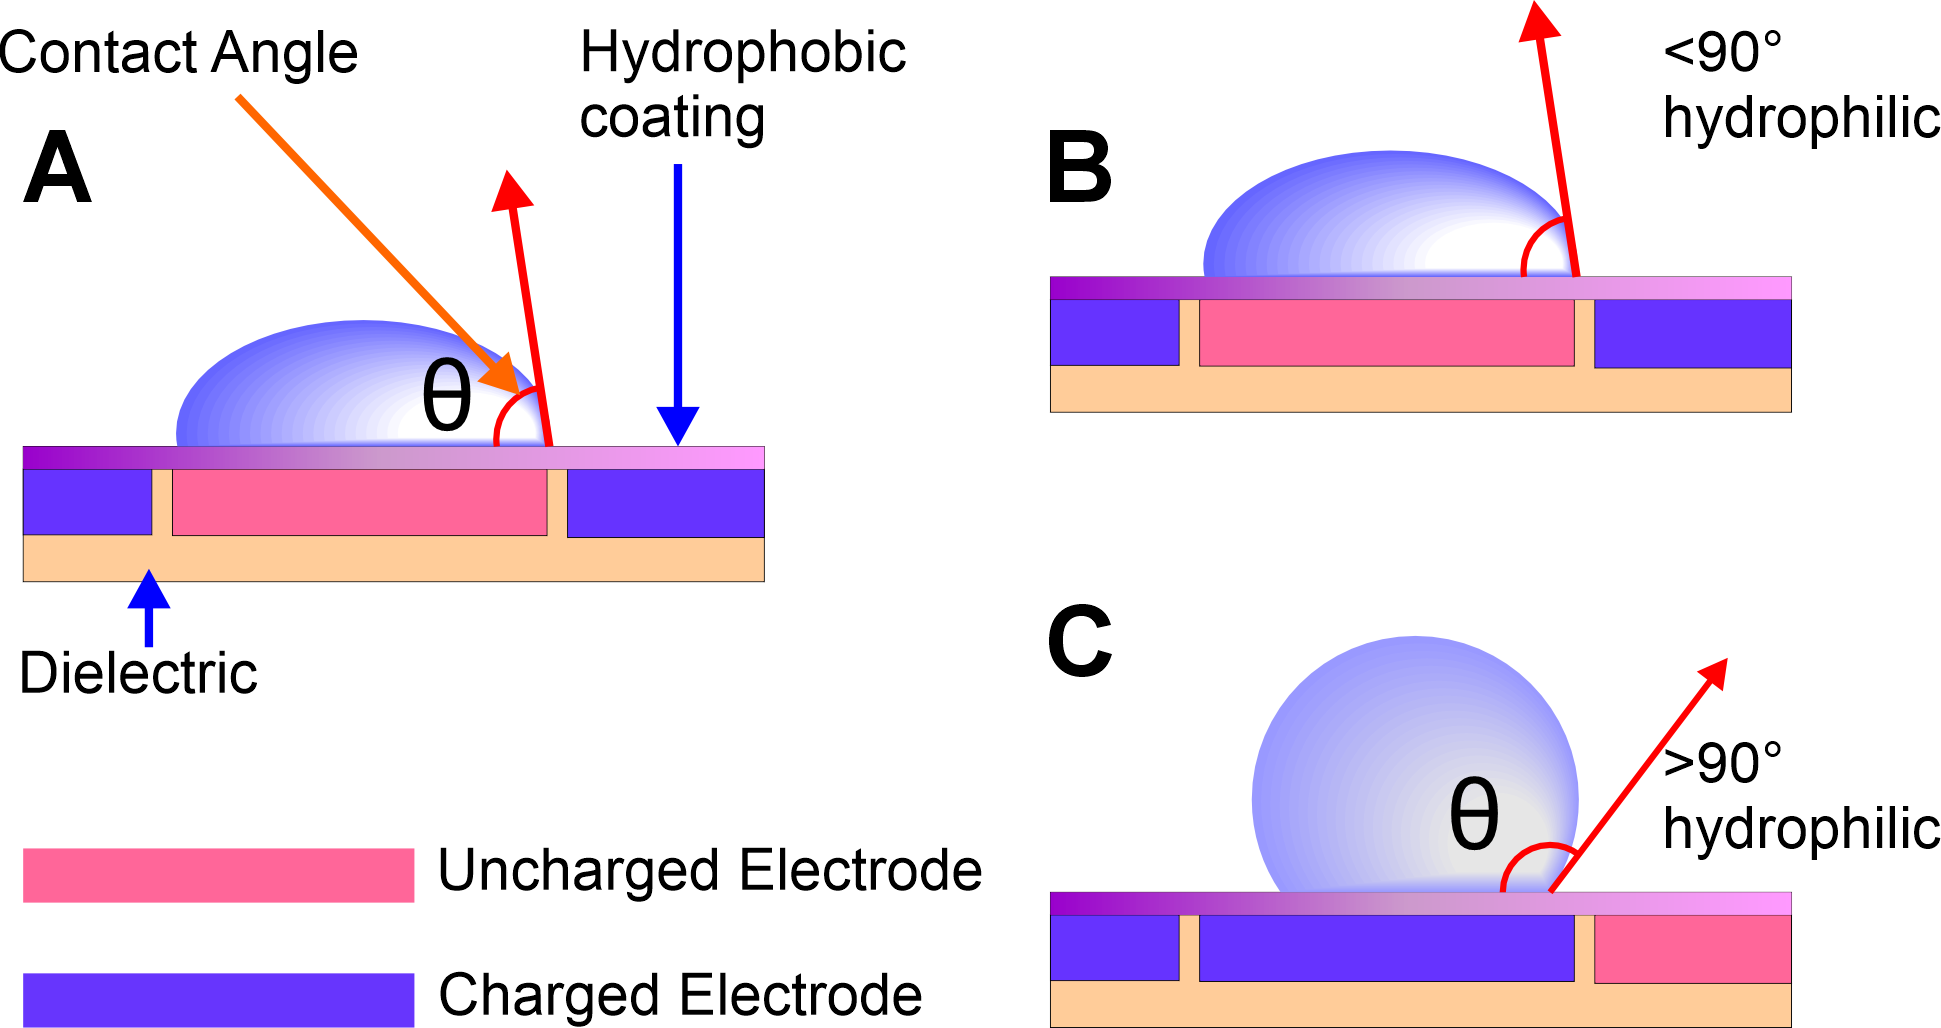
\includegraphics[width=\columnwidth]{ContactAngle.png}
    \caption{Contact angle of a droplet on a solid surface \cite{kothamachuRoleDigitalMicrofluidics2020}.}
    \label{contactangle}
\end{figure}

The Young’s equation describes the balance of forces at the three-phase contact line, relating the contact angle ($\theta$) to the interfacial tensions as shown in Equation \ref{Young–Lippmann_V1} \cite{banerjeeDeterministicSplittingFluid2012,basuDevelopmentGrapheneOxide2021}.
\begin{equation}
\label{Young–Lippmann_V1}
\cos~(\theta_{V}) = \cos~(\theta_{0})~+~\frac{\epsilon_{r}\epsilon_{0}V^{2}}{2\gamma_{LG}d}
\end{equation}

\noindent where $\theta_{V}$ is the contact angle under applied voltage, $\theta_{0}$ is the equilibrium contact angle, $\epsilon_{r}$ is the relative permittivity of the dielectric layer, $\epsilon_{0}$ is the vacuum permittivity, $V$ is the applied voltage, $\gamma_{LG}$ is the liquid-gas interfacial tension, and $d$ is the thickness of the dielectric layer.

This equation highlights the inverse square relationship between contact angle change and dielectric thickness, and the direct square relationship with applied voltage and dielectric constant. Optimising these parameters is crucial for achieving low-voltage, reliable droplet actuation, particularly important for portable and disposable PCB-based platform. To visualize this relationship, Figure \ref{Young–Lippmann} illustrates the contact angle variation with applied voltage for a dielectric layer of thickness $d$ and relative permittivity $\epsilon_{r}$.
\begin{figure}[h!]
    \centering
    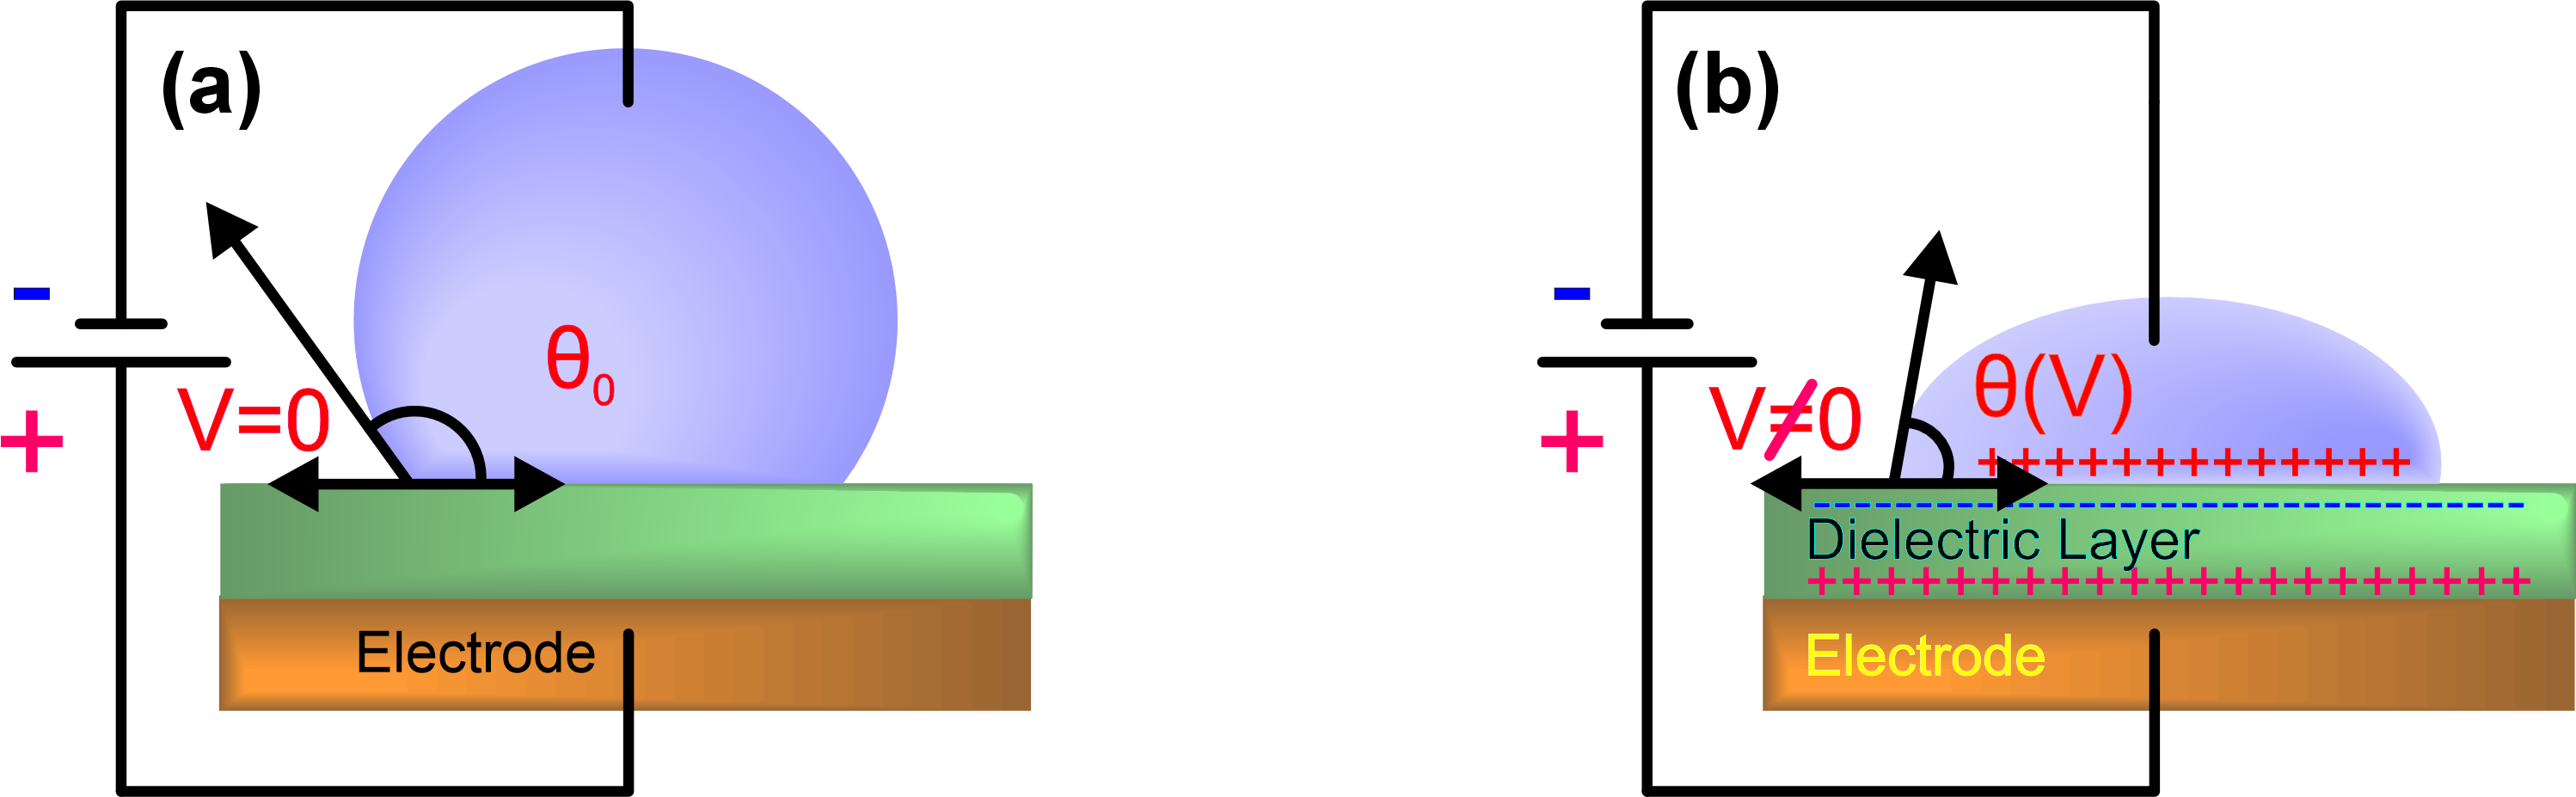
\includegraphics[width=\columnwidth]{ContactAngleWhenActuated.png}
    \caption{Droplet contact angle variation with applied voltage \cite{jainDesignFabricationCharacterization2017}.}
    \label{Young–Lippmann}
\end{figure}

However, the equation assumes a single dielectric layer, which is often not the case in practical applications where multiple dielectric layers are present. To accurately represent this multi-layered system, the concept of an equivalent capacitance per unit area ($C_{eff}$) must be employed. For multiple dielectric layers in series, the reciprocal of the total effective capacitance is the sum of the reciprocals of the individual layer capacitances.

Consider a common scenario with two distinct insulating layers:
\begin{enumerate}
    \item  A dielectric layer (e.g., SU-8, \(\ce{Si3N4}\)) with thickness $d_d$ and relative permittivity $\epsilon{r,d}$.
    \item A hydrophobic layer (e.g., Teflon, PDMS) with thickness $d_h$ and relative permittivity $\epsilon_{r,h}$.
\end{enumerate}

The capacitance per unit area for each individual layer is shown in Equation \ref{Capacitance2Materials}.

\begin{equation}
\begin{aligned}
\label{Capacitance2Materials}
C_{d} &= \frac{\epsilon_{r,d}\epsilon_{0}}{d_d} \\
C_{h} &= \frac{\epsilon_{r,h}\epsilon_{0}}{d_h}
\end{aligned}
\end{equation}

Therefore, the effective capacitance per unit area ($C_{eff}$) for the two layers in series is given by Equation \ref{Capacitance2MaterialsSeries}.
\begin{equation}
\label{Capacitance2MaterialsSeries}
 C_{eff} = \frac{\epsilon_0}{\frac{d_d}{\epsilon_{r,d}} + \frac{d_h}{\epsilon_{r,h}}}
\end{equation}

Finally, the effective capacitance can be used to calculate the contact angle variation under applied voltage using the expanded Young–Lippmann equation as shown in Equation \ref{Young–Lippmann_V2}.
\begin{equation}
\label{Young–Lippmann_V2}
\cos \theta_{V} = \cos \theta_{0} + \frac{\epsilon_{0}}{2\gamma_{LG} \left(\frac{d_{d}}{\epsilon_{r,d}} + \frac{d_{h}}{\epsilon_{r,h}}\right)} V^{2}
\end{equation}

This specific form is directly supported by the literature, where researchers like Bhattacharjee and Najjaran present a similar equation for two layers (hydrophobic and dielectric) in series, influencing the contact angle change \cite{bhattacharjeeDropletPositionControl2010}. This equation demonstrates that the overall electrical performance of the dielectric stack, and consequently the EWOD actuation, is governed by the combined electrical impedance of both layers.

\section{Proposed Simulation Methodology}

The simulation of droplet contact angle measurement against varying applied DC voltage was conducted using COMSOL Multiphysics, a powerful finite element analysis software. The simulation setup involved the following subsections.

\subsection{Physics Modules and Study Selection}
The simulation utilized the \textit{Electrostatics} and \textit{Moving Mesh} modules to model the electrostatic forces acting on the droplet and the movement of the contact line. The study type was set to \textit{Stationary} to analyze the droplet behavior under static conditions with varying applied voltages.
\subsection{Geometry Creation}
The geometry of the droplet and the substrate was created in COMSOL, ensuring accurate representation of the droplet shape and the surface features.
\subsection{Material Properties}
The material properties, including the dielectric constant and interfacial tension, were defined based on the materials used in the experiment.
\subsection{Boundary Conditions}
Appropriate boundary conditions were applied to simulate the contact angle and the influence of the applied voltage on the droplet behavior.
\subsection{Mesh Generation}
A fine mesh was generated to ensure accurate numerical results, particularly around the contact line where gradients are steep.
\subsection{Simulation Execution}
he simulation was executed, varying the applied DC voltage to observe changes in the contact angle.
\subsection{Post-Processing}
The results were post-processed to extract the contact angle values and visualize the droplet behavior under different voltage conditions.

\section{Simulation Challenges Encountered}

\section{Conclusion}

\section{Acknowledgement}
The authors gratefully acknowledge the support from
the Ministry of Higher Education Malaysia for Fundamental
Research Grant Scheme with Project Code:
FRGS/1/2022/TK0/USM/02/10.



%----------------------------------------------------------

\printbibliography

%----------------------------------------------------------

\end{document}